%%%%%%%%%%%%%%
%% Run LaTeX on this file several times to get Table of Contents,
%% cross-references, and citations.

%% If you have font problems, you may edit the w-bookps.sty file
%% to customize the font names to match those on your system.

%% w-bksamp.tex. Current Version: Feb 16, 2012
%%%%%%%%%%%%%%%%%%%%%%%%%%%%%%%%%%%%%%%%%%%%%%%%%%%%%%%%%%%%%%%%
%
%  Sample file for
%  Wiley Book Style, Design No.: SD 001B, 7x10
%  Wiley Book Style, Design No.: SD 004B, 6x9
%
%
%  Prepared by Amy Hendrickson, TeXnology Inc.
%  http://www.texnology.com
%%%%%%%%%%%%%%%%%%%%%%%%%%%%%%%%%%%%%%%%%%%%%%%%%%%%%%%%%%%%%%%%

%%%%%%%%%%%%%
% 7x10
%\documentclass{wileySev}

% 6x9
\documentclass{wileySix}

\usepackage{graphicx}
\usepackage{listings}
\usepackage{float}
\usepackage[urlcolor=blue, colorlinks=true]{hyperref}
\usepackage{textcomp}
\usepackage{color}
 
\definecolor{codegreen}{rgb}{0,0.6,0}
\definecolor{codegray}{rgb}{0.5,0.5,0.5}
\definecolor{codepurple}{rgb}{0.58,0,0.82}
\definecolor{backcolour}{rgb}{0.95,0.95,0.92}
 
\lstdefinestyle{mystyle}{
    backgroundcolor=\color{backcolour},   
    commentstyle=\color{codegreen},
    keywordstyle=\color{magenta},
    numberstyle=\tiny\color{codegray},
    stringstyle=\color{codepurple},
    basicstyle=\footnotesize,
    breakatwhitespace=false,         
    breaklines=true,                 
    captionpos=b,                    
    keepspaces=true,                 
    numbers=left,                    
    numbersep=5pt,                  
    showspaces=false,                
    showstringspaces=false,
    showtabs=false,                  
    tabsize=2,
    language=sh
}
 
\lstset{style=mystyle}

%%%%%%%
%% for times math: However, this package disables bold math (!)
%% \mathbf{x} will still work, but you will not have bold math
%% in section heads or chapter titles. If you don't use math
%% in those environments, mathptmx might be a good choice.

% \usepackage{mathptmx}

% For PostScript text
%\usepackage{w-bookps}

%%%%%%%%%%%%%%%%%%%%%%%%%%%%%%%%%%%%%%%%%%%%%%%%%%%%%%%%%%%%%%%%
%% Other packages you might want to use:

% for chapter bibliography made with BibTeX
% \usepackage{chapterbib}

% for multiple indices
% \usepackage{multind}

% for answers to problems
% \usepackage{answers}

%%%%%%%%%%%%%%%%%%%%%%%%%%%%%%
%% Change options here if you want:
%%
%% How many levels of section head would you like numbered?
%% 0= no section numbers, 1= section, 2= subsection, 3= subsubsection
%%==>>
\setcounter{secnumdepth}{3}

%% How many levels of section head would you like to appear in the
%% Table of Contents?
%% 0= chapter titles, 1= section titles, 2= subsection titles, 
%% 3= subsubsection titles.
%%==>>
\setcounter{tocdepth}{2}

%% Cropmarks? good for final page makeup
%% \docropmarks

%%%%%%%%%%%%%%%%%%%%%%%%%%%%%%
%
% DRAFT
%
% Uncomment to get double spacing between lines, current date and time
% printed at bottom of page.
% \draft
% (If you want to keep tables from becoming double spaced also uncomment
% this):
% \renewcommand{\arraystretch}{0.6}
%%%%%%%%%%%%%%%%%%%%%%%%%%%%%%

%%%%%%% Demo of section head containing sample macro:
%% To get a macro to expand correctly in a section head, with upper and
%% lower case math, put the definition and set the box 
%% before \begin{document}, so that when it appears in the 
%% table of contents it will also work:

\newcommand{\VT}[1]{\ensuremath{{V_{T#1}}}}

%% use a box to expand the macro before we put it into the section head:

\newbox\sectsavebox
\setbox\sectsavebox=\hbox{\boldmath\VT{xyz}}

%%%%%%%%%%%%%%%%% End Demo


\begin{document}


\booktitle{Cerdas Menguasai Git}
\subtitle{Dalam 24 Jam}

\authors{Rolly M. Awangga\\
\affil{Informatics Research Center}
%Floyd J. Fowler, Jr.\\
%\affil{University of New Mexico}
}

\offprintinfo{Cerdas Menguasai Git, First Edition}{Rolly M. Awangga}

%% Can use \\ if title, and edition are too wide, ie,
%% \offprintinfo{Survey Methodology,\\ Second Edition}{Robert M. Groves}

%%%%%%%%%%%%%%%%%%%%%%%%%%%%%%
%% 
\halftitlepage

\titlepage


\begin{copyrightpage}{2019}
%Survey Methodology / Robert M. Groves . . . [et al.].
%\       p. cm.---(Wiley series in survey methodology)
%\    ``Wiley-Interscience."
%\    Includes bibliographical references and index.
%\    ISBN 0-471-48348-6 (pbk.)
%\    1. Surveys---Methodology.  2. Social 
%\  sciences---Research---Statistical methods.  I. Groves, Robert M.  II. %
%Series.\\
%
%HA31.2.S873 2007
%001.4'33---dc22                                             2004044064
\end{copyrightpage}

\dedication{`Jika Kamu tidak dapat menahan lelahnya belajar, 
Maka kamu harus sanggup menahan perihnya Kebodohan.'
~Imam Syafi'i~}

\begin{contributors}
\name{Rolly Maulana Awangga,} Informatics Research Center., Politeknik Pos Indonesia, Bandung,
Indonesia



\end{contributors}

\contentsinbrief
\tableofcontents
\listoffigures
\listoftables
\lstlistoflistings


\begin{foreword}
Sepatah kata dari Kaprodi, Kabag Kemahasiswaan dan Mahasiswa
\end{foreword}

\begin{preface}
Buku ini diciptakan bagi yang awam dengan git sekalipun.

\prefaceauthor{R. M. Awangga}
\where{Bandung, Jawa Barat\\
Februari, 2019}
\end{preface}


\begin{acknowledgments}
Terima kasih atas semua masukan dari para mahasiswa agar bisa membuat buku ini 
lebih baik dan lebih mudah dimengerti.

Terima kasih ini juga ditujukan khusus untuk team IRC yang 
telah fokus untuk belajar dan memahami bagaimana buku ini mendampingi proses 
Intership.
\authorinitials{R. M. A.}
\end{acknowledgments}

\begin{acronyms}
\acro{ACGIH}{American Conference of Governmental Industrial Hygienists}
\acro{AEC}{Atomic Energy Commission}
\acro{OSHA}{Occupational Health and Safety Commission}
\acro{SAMA}{Scientific Apparatus Makers Association}
\end{acronyms}

\begin{glossary}
\term{git}Merupakan manajemen sumber kode yang dibuat oleh linus torvald.

\term{bash}Merupakan bahasa sistem operasi berbasiskan *NIX.

\term{linux}Sistem operasi berbasis sumber kode terbuka yang dibuat oleh Linus Torvald
\end{glossary}

\begin{symbols}
\term{A}Amplitude

\term{\hbox{\&}}Propositional logic symbol 

\term{a}Filter Coefficient

\bigskip

\term{\mathcal{B}}Number of Beats
\end{symbols}

\begin{introduction}

%% optional, but if you want to list author:

\introauthor{Rolly Maulana Awangga, S.T., M.T.}
{Informatics Research Center\\
Bandung, Jawa Barat, Indonesia}

Pada era disruptif  \index{disruptif}\index{disruptif!modern} 
saat ini. git merupakan sebuah kebutuhan dalam sebuah organisasi pengembangan perangkat lunak.
Buku ini diharapkan bisa menjadi penghantar para programmer, analis, IT Operation dan Project Manajer.
Dalam melakukan implementasi git pada diri dan organisasinya.

Rumusnya cuman sebagai contoh aja biar keren\cite{awangga2018sampeu}.

\begin{equation}
ABC {\cal DEF} \alpha\beta\Gamma\Delta\sum^{abc}_{def}
\end{equation}

\end{introduction}

%%%%%%%%%%%%%%%%%%Isi Buku_

\chapter{Chapter 1}
\section{1174006 - Kadek Diva Krishna Murti}
Lorem ipsum dolor sit amet, consectetur adipiscing elit.

\lstinputlisting[firstline=1, lastline=8]{references.bib}
\hfill\break
\begin{figure}[H]
    
\includegraphics[width=4cm]{kreatiflogo.png}
    \centering
    \caption{Kecerdasan Buatan.}
\end{figure}

\begin{enumerate}
	\item Lorem ipsum dolor sit amet, consectetur adipiscing elit.
	\item Lorem ipsum dolor sit amet, consectetur adipiscing elit.
	\item Lorem ipsum dolor sit amet, consectetur adipiscing elit.
\end{enumerate}

\subsection{Teori}

\subsection{Praktek}

\subsection{Penanganan Error}

\subsection{Bukti Tidak Plagiat}
\begin{figure}[H]
	
\includegraphics[width=4cm]{kreatiflogo.png}
	\centering
	\caption{Kecerdasan Buatan.}
\end{figure}
\section{Fanny Shafira Damayanti (1174069)}
\subsection{Teori}
\begin{enumerate}
\item Definisi Kecerdasan buatan\\ 
Kecerdasan buatan atau Artificial intelligence merupakan kecerdasan yang ditambahkkan kedalam suatu system yang diatur secara ilmiah. Kecerdasan buatan dibuat untuk menggantikan pekerjaan yang dilakukan oleh manusia menjadi dikerjakan oleh sistem.

\item Sejarah Kecerdasan Buatan
\begin{itemize}
\item Abad 17, Rene Descartes berkata bahwa tubuh hewan adalah sekumpulan mesin yang rumit.
\item 1642, Blaise Pascal menciptakan mesin penghitung digital mekanis pertama.
\item Abad 19, Charles Babbage dan Ada Lovelace bekerja di program penghitung mekanis.
\item 1950, John McCarthy membuat istilah “Kecerdasan Buatan”.
\item 1960-1970, Joel Moses membuat program yang pertama kali sukses dalam bidang matematika.
\item 1980, jaringan saraf digunakan secara meluas dengan algoritme perambatan balik.
\item 2004, DARPA membuat kendaraan yang bisa dijalankan sendiri tanpa manusia.
\end{itemize}

\item Perkembangan kecerdasan buatan
\begin{itemize}
\item Masa persiapan (1943-1946)
Warren McCulloch dan Walter Pitt mengemukakan tiga hal : pengetahuan fisiologi dasar dan fungsi sel syaraf dalam otak, analisa formal tentang logika proposisi, dan teori komputasi Turing.

Pada tahun 1950, Nobert Wiener membuat penelitian mengenai prinsip-prinsip teori feedback.

Pada tahun 1956, John McCarthy meyakinkan Minsky, Claude Shannon dan Nathaniel Rochester untuk membantunya melakukan penelitian dalam bidan Otomata, Jaringan Syaraf dan pembelajaran intelijensia. 

\item Awal perkembangan (1952-1969)
Pada tahun 1958, McCarthy di MIT AI Lab Memo No.1 mendefinisikan bahasa pemrograman tingkat tinggi yaitu LISP,

Pada tahun 1959, Nathaniel Rochester dari IBM dan mahasiswa-mahasiswanya mengeluarkan program kecerdasan buatan yaitu Geometry Theorm Prover.

Pada tahun 1963, program yang dibuat James Slagle mampu menyelesaikan masalah integral tertutup untuk mata kuliah Kalkulus.
Pada tahun 1986, program analogi buatan Tom Evan menyelesaikan masalah analogi geometris yang ada pada tes IQ.

\item Perkembangan Kecerdasan Buatan Melambat (1969-1979)
Bruce Buchanan dan Joshua Lederberg yang membuat program untuk memecahkan masalah struktur molekul dari informasi yang didapatkan dari spectrometer massa.

\item AI Menjadi sebuah industri
Industrialisasi kecerdasan buatan diawali dengan ditemukannya sistem pakar yang dinamakan R1 yang mampu mengkonfigurasi system-sistem computer baru. 

\item Kembalinya Jaringan Syaraf Tiruan (1986-sekarang)
Pada tahun 1985-an setidaknya empat kelompok riset menemukan kembali algoritma belajar propagasi balik (Black-Propagation Learning). Algoritma ini berhasil diimplementasikan ke dalam bidang ilmu computer dan psikologi.
\end{itemize}

\item Definisi Supervised Learning\\
Supervised Learning merupakan cabang dari Artificial Intelligence. supervised learning adalah suatu ilmu yang mempelajari perancangan dan pengembangan algoritma.

\item Klasifikasi Supervised Learning
\begin{itemize}
\item Logistic regression.
\item K-nearest neighbors.
\item Support vector machine (SVM)
\item Naive Bayes.
\item Decision tree classification.
\item Random forest classification.
\end{itemize}

\item Regresi dan Unsupervised Learning\\
Regresi merupakan sebuah metode analisis statistic yang digunkan untuk mengetahui pengaruh antara dua variable atau lebih.

Untuk mempelajari Unsupervised learning kita tidak perlu data training untuk melakukan prediksi maupun klasifikasi.

\item Dataset\\
Dataset merupakan objek yang mempresentasikan data dan relasinya pada memori.

\item Training Set\\
Training Set merupakan bagian dari dataset untuk membuat prediksi atau menjalankan fungsi dari sebuah algoritma Machine Learning.

\item Testing Set\\
Testing set digunakan untuk mengukur apakah classifier berhasil melakukan klasifikasi dengan benar.

\end{enumerate}

\subsection{Instalasi}
\begin{enumerate}
	\item Instalasi Library scikit dari anaconda, mencoba kompilasi dan uji coba ambil contoh kode dan lihat variabel explorer
	\hfill\break
	\begin{figure}[H]
		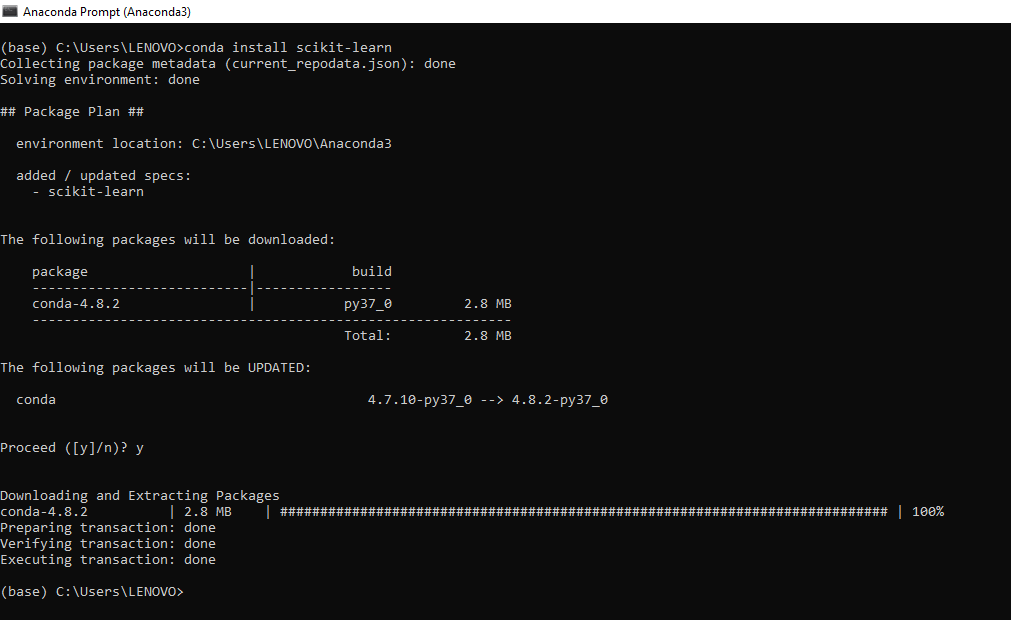
\includegraphics[width=4cm]{figures/1174069/1/1.png}
		\centering
		\caption{Instalasi Package Scikit Learn}
	\end{figure}
	\begin{figure}[H]
		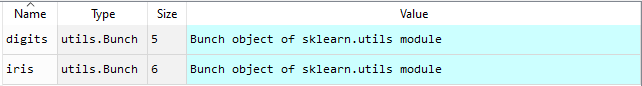
\includegraphics[width=4cm]{figures/1174069/1/2.png}
		\centering
		\caption{Isi Variabel Explorer}
	\end{figure}
	\item Mencoba Loading an example dataset, menjelaskan maksud dari tulisan tersebut dan mengartikan           		  per baris
	\hfill\break
	\lstinputlisting[firstline=7, lastline=11]{src/1174069/1/1174069.py}
	\item Mencoba Learning and predicting, menjelaskan maksud dari tulisan tersebut dan mengartikan per  			  baris
	\hfill\break
	\lstinputlisting[firstline=13, lastline=22]{src/1174069/1/1174069.py}
	\item  Mencoba Model persistence, menjelaskan maksud dari tulisan tersebut dan mengartikan per baris
	\hfill\break
	\lstinputlisting[firstline=25, lastline=34]{src/1174069/1/1174069.py}
	\item Mencoba Conventions, menjelaskan maksud dari tulisan tersebut dan mengartikan per baris
	\hfill\break
	\lstinputlisting[firstline=37, lastline=48]{src/1174069/1/1174069.py}
\end{enumerate}

\subsection{Penanganan Error}
\begin{enumerate}
	\item ScreenShoot Error
	\begin{figure}[H]
		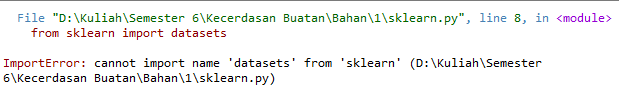
\includegraphics[width=4cm]{figures/1174069/1/error/1.png}
		\centering
		\caption{Import Error}
	\end{figure}

	\item Tuliskan Kode Error dan Jenis Error
	\begin{itemize}
		\item Import Error
	\end{itemize}
	\item Cara Penangan Error
	\begin{itemize}
		\item Import Error
		\hfill\break
		Dengan Menginstall Library Yang Tidak Ditemukan
	\end{itemize}
\end{enumerate}

\subsection{Bukti Tidak Plagiat}
\begin{figure}[H]
	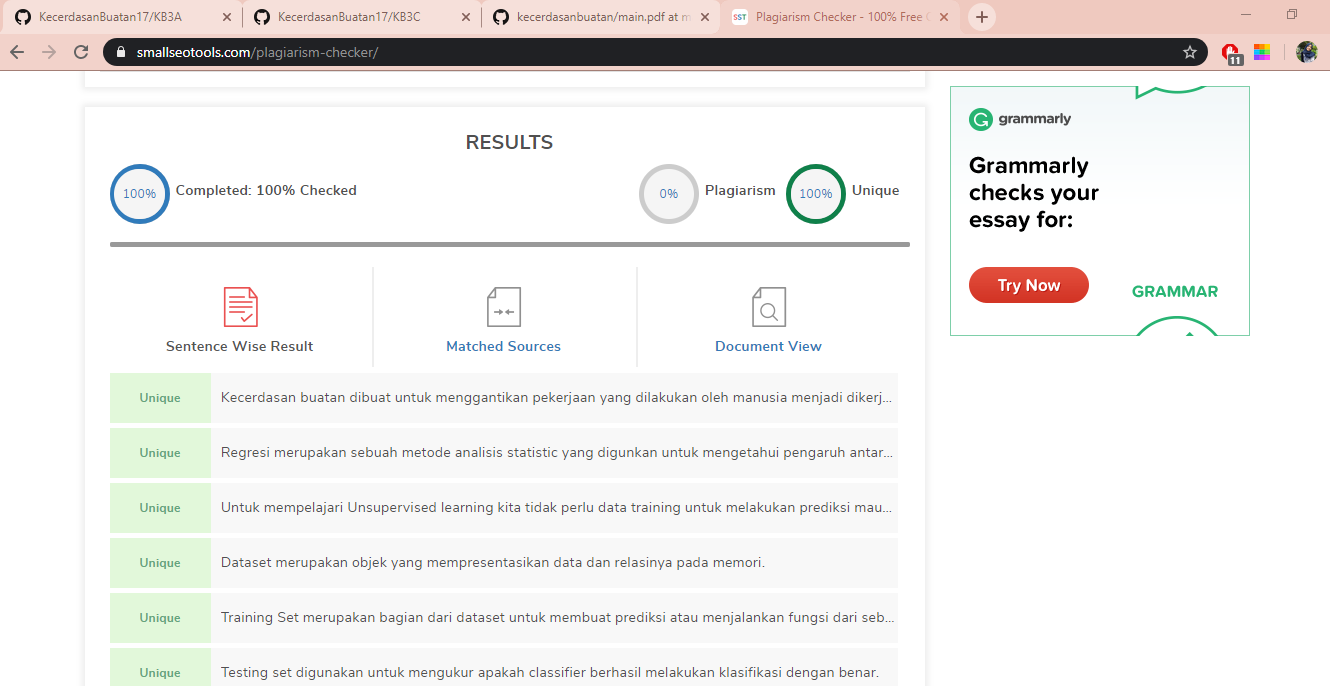
\includegraphics[width=4cm]{figures/1174069/1/plagiat/plagiat.png}
	\centering
	\caption{Bukti Tidak Melakukan Plagiat Chapter 1}
\end{figure}

\subsection{Link Youtube}



\chapter{Chapter 2}
\section{1174006 - Kadek Diva Krishna Murti}
Lorem ipsum dolor sit amet, consectetur adipiscing elit.

\lstinputlisting[firstline=1, lastline=8]{references.bib}
\hfill\break
\begin{figure}[H]
    
\includegraphics[width=4cm]{kreatiflogo.png}
    \centering
    \caption{Kecerdasan Buatan.}
\end{figure}

\begin{enumerate}
	\item Lorem ipsum dolor sit amet, consectetur adipiscing elit.
	\item Lorem ipsum dolor sit amet, consectetur adipiscing elit.
	\item Lorem ipsum dolor sit amet, consectetur adipiscing elit.
\end{enumerate}

\subsection{Teori}

\subsection{Praktek}

\subsection{Penanganan Error}

\subsection{Bukti Tidak Plagiat}
\begin{figure}[H]
	
\includegraphics[width=4cm]{kreatiflogo.png}
	\centering
	\caption{Kecerdasan Buatan.}
\end{figure}

\chapter{Chapter 3}
\section{1174006 - Kadek Diva Krishna Murti}
Lorem ipsum dolor sit amet, consectetur adipiscing elit.

\lstinputlisting[firstline=1, lastline=8]{references.bib}
\hfill\break
\begin{figure}[H]
    
\includegraphics[width=4cm]{kreatiflogo.png}
    \centering
    \caption{Kecerdasan Buatan.}
\end{figure}

\begin{enumerate}
	\item Lorem ipsum dolor sit amet, consectetur adipiscing elit.
	\item Lorem ipsum dolor sit amet, consectetur adipiscing elit.
	\item Lorem ipsum dolor sit amet, consectetur adipiscing elit.
\end{enumerate}

\subsection{Teori}

\subsection{Praktek}

\subsection{Penanganan Error}

\subsection{Bukti Tidak Plagiat}
\begin{figure}[H]
	
\includegraphics[width=4cm]{kreatiflogo.png}
	\centering
	\caption{Kecerdasan Buatan.}
\end{figure}

\chapter{Chapter 4}
\section{1174006 - Kadek Diva Krishna Murti}
Lorem ipsum dolor sit amet, consectetur adipiscing elit.

\lstinputlisting[firstline=1, lastline=8]{references.bib}
\hfill\break
\begin{figure}[H]
    
\includegraphics[width=4cm]{kreatiflogo.png}
    \centering
    \caption{Kecerdasan Buatan.}
\end{figure}

\begin{enumerate}
	\item Lorem ipsum dolor sit amet, consectetur adipiscing elit.
	\item Lorem ipsum dolor sit amet, consectetur adipiscing elit.
	\item Lorem ipsum dolor sit amet, consectetur adipiscing elit.
\end{enumerate}

\subsection{Teori}

\subsection{Praktek}

\subsection{Penanganan Error}

\subsection{Bukti Tidak Plagiat}
\begin{figure}[H]
	
\includegraphics[width=4cm]{kreatiflogo.png}
	\centering
	\caption{Kecerdasan Buatan.}
\end{figure}

\chapter{Chapter 5}
\section{1174006 - Kadek Diva Krishna Murti}
Lorem ipsum dolor sit amet, consectetur adipiscing elit.

\lstinputlisting[firstline=1, lastline=8]{references.bib}
\hfill\break
\begin{figure}[H]
    
\includegraphics[width=4cm]{kreatiflogo.png}
    \centering
    \caption{Kecerdasan Buatan.}
\end{figure}

\begin{enumerate}
	\item Lorem ipsum dolor sit amet, consectetur adipiscing elit.
	\item Lorem ipsum dolor sit amet, consectetur adipiscing elit.
	\item Lorem ipsum dolor sit amet, consectetur adipiscing elit.
\end{enumerate}

\subsection{Teori}

\subsection{Praktek}

\subsection{Penanganan Error}

\subsection{Bukti Tidak Plagiat}
\begin{figure}[H]
	
\includegraphics[width=4cm]{kreatiflogo.png}
	\centering
	\caption{Kecerdasan Buatan.}
\end{figure}

\chapter{Chapter 6}
\section{1174006 - Kadek Diva Krishna Murti}
Lorem ipsum dolor sit amet, consectetur adipiscing elit.

\lstinputlisting[firstline=1, lastline=8]{references.bib}
\hfill\break
\begin{figure}[H]
    
\includegraphics[width=4cm]{kreatiflogo.png}
    \centering
    \caption{Kecerdasan Buatan.}
\end{figure}

\begin{enumerate}
	\item Lorem ipsum dolor sit amet, consectetur adipiscing elit.
	\item Lorem ipsum dolor sit amet, consectetur adipiscing elit.
	\item Lorem ipsum dolor sit amet, consectetur adipiscing elit.
\end{enumerate}

\subsection{Teori}

\subsection{Praktek}

\subsection{Penanganan Error}

\subsection{Bukti Tidak Plagiat}
\begin{figure}[H]
	
\includegraphics[width=4cm]{kreatiflogo.png}
	\centering
	\caption{Kecerdasan Buatan.}
\end{figure}

\chapter{Chapter 7}
\section{1174006 - Kadek Diva Krishna Murti}
Lorem ipsum dolor sit amet, consectetur adipiscing elit.

\lstinputlisting[firstline=1, lastline=8]{references.bib}
\hfill\break
\begin{figure}[H]
    
\includegraphics[width=4cm]{kreatiflogo.png}
    \centering
    \caption{Kecerdasan Buatan.}
\end{figure}

\begin{enumerate}
	\item Lorem ipsum dolor sit amet, consectetur adipiscing elit.
	\item Lorem ipsum dolor sit amet, consectetur adipiscing elit.
	\item Lorem ipsum dolor sit amet, consectetur adipiscing elit.
\end{enumerate}

\subsection{Teori}

\subsection{Praktek}

\subsection{Penanganan Error}

\subsection{Bukti Tidak Plagiat}
\begin{figure}[H]
	
\includegraphics[width=4cm]{kreatiflogo.png}
	\centering
	\caption{Kecerdasan Buatan.}
\end{figure}

\bibliographystyle{IEEEtran} 
%\def\bibfont{\normalsize}
\bibliography{references}


%%%%%%%%%%%%%%%
%%  The default LaTeX Index
%%  Don't need to add any commands before \begin{document}
\printindex

%%%% Making an index
%% 
%% 1. Make index entries, don't leave any spaces so that they
%% will be sorted correctly.
%% 
%% \index{term}
%% \index{term!subterm}
%% \index{term!subterm!subsubterm}
%% 
%% 2. Run LaTeX several times to produce <filename>.idx
%% 
%% 3. On command line, type  makeindx <filename> which
%% will produce <filename>.ind 
%% 
%% 4. Type \printindex to make the index appear in your book.
%% 
%% 5. If you would like to edit <filename>.ind 
%% you may do so. See docs.pdf for more information.
%% 
%%%%%%%%%%%%%%%%%%%%%%%%%%%%%%

%%%%%%%%%%%%%% Making Multiple Indices %%%%%%%%%%%%%%%%
%% 1. 
%% \usepackage{multind}
%% \makeindex{book}
%% \makeindex{authors}
%% \begin{document}
%% 
%% 2.
%% % add index terms to your book, ie,
%% \index{book}{A term to go to the topic index}
%% \index{authors}{Put this author in the author index}
%% 
%% \index{book}{Cows}
%% \index{book}{Cows!Jersey}
%% \index{book}{Cows!Jersey!Brown}
%% 
%% \index{author}{Douglas Adams}
%% \index{author}{Boethius}
%% \index{author}{Mark Twain}
%% 
%% 3. On command line type 
%% makeindex topic 
%% makeindex authors
%% 
%% 4.
%% this is a Wiley command to make the indices print:
%% \multiprintindex{book}{Topic index}
%% \multiprintindex{authors}{Author index}

\end{document}

